\chapter{Anexo}
\label{cap:capitulo9}

\begin{flushright}
\begin{minipage}[]{10cm}
\emph{Las ideas no duran mucho. Hay que hacer algo con ellas}\\
\end{minipage}\\

Santiago Ramón y Cajal\\
\end{flushright}

\vspace{1cm}

En este anexo se van a tratar los pasos necesarios para conseguir replicar este proyecto.

\section{Construcción del robot} 
\label{subsec:anexoconstruccion}

%incluir enlace del tutorial de construir el robot en físico


\section{Ejecución del robot en simulación}
\label{subsec:anexosimulacion}

Es necesario instalar los siguientes programas: 

\begin{verbatim}
	sudo apt update && sudo apt upgrade
	sudo apt install ros-humble-ros2-control ros-humble-ros2-controllers
	sudo apt install ros-humble-rviz2
	sudo apt install ros-humble-gazebo-ros-pkgs
	sudo apt install ros-humble-xacro ros-humble-robot-state-publisher 
	sudo apt install ros-humble-joint-state-publisher
\end{verbatim}
 
Una vez instalado los programas, es el momento de ponerlo en ejecución y para ello, únicamente hay que escribir los siguientes comandos:
\begin{verbatim}
	colcon build --packages-select pibotj_r2c   # compila los paquetes
	source ./install/setup.bash                 # configura variables 
	ros2 launch pibotj_r2c launch_sim.launch.py
\end{verbatim} 

Si la primera vez que se lance el robot ocurre algún error, es normal y hay que reiniciar el proceso.

\section{Configuración del robot real}
\label{subsec:anexoconfig}

En este apartado es importante instalar Ubuntu 20.04 y ROS 2 Foxy en vez de simulación que fue Ubuntu 22.04 y ROS2 Humble (como se puede ver en el apartado anterior).
 
Se va a trabajar conectándose por ssh al robot, escribiendo \verb|ssh usuario@ip_dispositivo| y posteriormente, introduciendo la constraseña creada en el proceso de instalación. Esta era la forma de comunicación con el robot ya que esta distribución, no tenía interfaz gráfica. De las variante de ssh se usaba scp -r para copiar directorios entre el robot y el ordenador local y permitir subir los cambios a Github, y para desarrollar código se usaba un \textit{plugin} de VSCode que permite usar VSCode conectándose al robot usando ssh\footnote{\url{https://code.visualstudio.com/docs/remote/ssh-tutorial}}. 
 
En los siguientes apartados se detalla cómo se ha configurado cada dispositivo que conforma el PiBotJ.

\subsection{Cámara}
\label{subsec:anexocamara}

La cámara está conectada al puerto CSI y, para hacerla funcionar, se necesitan los siguientes programas: 

\begin{verbatim}
	sudo apt-get install gstreamer1.0-tools \ 
	gstreamer1.0-plugins-base gstreamer1.0-plugins-good \ 
	gstreamer1.0-plugins-bad gstreamer1.0-plugins-ugly
\end{verbatim}

Una vez instalados, fue necesario editar el fichero \verb|/boot/firmware/config.txt| añadiendo \verb|start_x=1| al final y se tuvo que reiniciar la Raspberry Pi. Para comprobar que la configuración fue correcta, era necesario usar el comando \verb|v4l2-ctl --list-devices|  que comprueba la lista de dispositivos de video y media que están disponibles en el sistema. En la Figura \ref{fig:v4l2} se puede ver el resultado de dicho comando y  muestra que la cámara se encontraba conectada en el dispositivo \verb|/dev/video0|.


\begin{figure} [h!]
	\begin{center}
		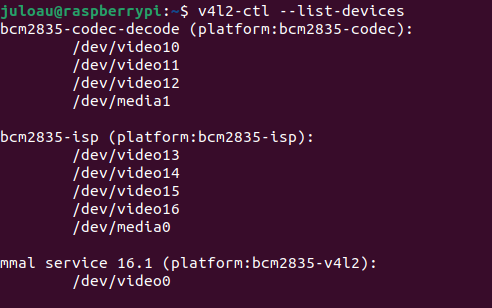
\includegraphics[width=9cm]{figs/cap6/vl.png}
	\end{center}
	\caption{Dispositivos de video y media disponibles en PiBotJ}
	\label{fig:v4l2}
\end{figure}


Sabiendo que la cámara estaba disponible, era necesario comprobar que realmente la imagen se pudiera ver correctamente.


\subsection{Google Coral}
\label{subsec:anexogooglecoral}

Se pueden encontrar diferentes pasos de instalación dependiendo de las necesidades del usuario, pero se pueden resumir para cumplir con las características de la arquitectura de este dispositivo de la siguiente manera:


\begin{lstlisting}[language=bash]
	echo "deb https://packages.cloud.google.com/apt \
	coral-edgetpu-stable main" | \
	sudo tee /etc/apt/sources.list.d/coral-edgetpu.list
	
	curl https://packages.cloud.google.com/apt/doc/apt-key.gpg \
	| sudo apt-key add -
	
	sudo apt-get update	
	sudo apt-get install libedgetpu1-std
	
	# Conecta el USB en uno de los puertos 3.0
	
	sudo apt-get install python3-pycoral
\end{lstlisting}

Finalmente, el proceso se debería haber completado cuando la salida del último comando se debería ver como muestra la Figura \ref{fig:outcoral}.

\begin{figure} [h!]
	\begin{center}
		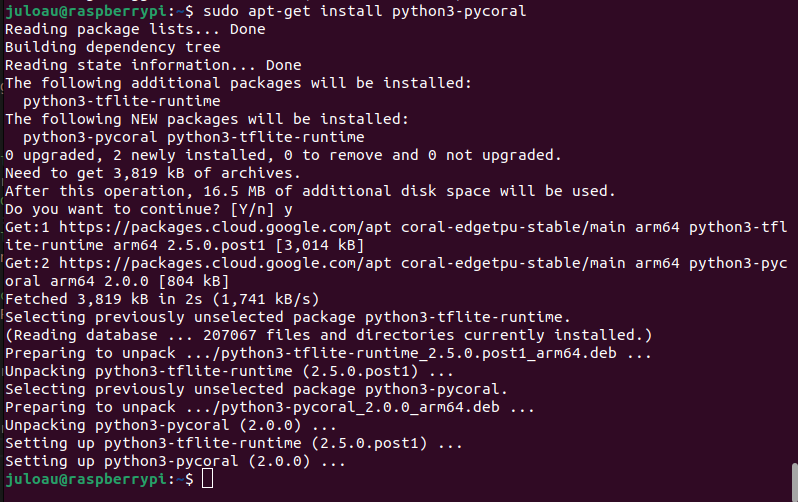
\includegraphics[width=12cm]{figs/cap6/pycoralinstalled.png}
	\end{center}
	\caption{Configuración exitosa del Google Coral}
	\label{fig:outcoral}
\end{figure} 

\subsection{Módulo GPS}
\label{subsec:anexogps}


La estructura seguida en este tutorial\footnote{\url{https://sparklers-the-makers.github.io/blog/robotics/use-neo-6m-module-with-raspberry-pi/}} ha sido de gran ayuda para configurar el módulo \acs{GPS} que, para esta arquitectura, supone seguir los siguientes pasos: 

Crea el fichero \verb|/etc/udev/rules.d/99-ttyAMA0.rules| que tiene que contener: \verb|KERNEL=="ttyAMA0", MODE="0666", GROUP="dialout"| y para que se actualicen en el sistema es necesario recargar las reglas, escribiendo por terminal lo siguiente: 

\begin{verbatim}
	sudo udevadm control --reload-rules
	sudo udevadm trigger
\end{verbatim}

Como esta distribución no tiene interfaz web, no tiene instalado por defecto \verb|raspi-config|. Así, para su instalación se ha seguido el siguiente tutorial\footnote{\url{https://github.com/EmilGus/install_raspi-config/tree/master}} y, una vez instalado, hay que ejecutarlo usando \verb|sudo raspi-config|. Dentro de \textit{raspi-config} hay que desplazarse hasta \textit{Interfacing options} y \textit{serial}, hay que desabilitar \textit{serial login shell}, habilitar \textit{serial interface} y reiniciar con \verb|sudo reboot|.

Finalmente los siguientes ficheros tienen que contener la siguiente información: 


\begin{lstlisting}[language=bash]
	cat /boot/firmware/config.txt 
	
	# Please DO NOT modify this file; if you need to modify the boot config,
	# the "usercfg.txt" file is the place to include user changes. Please 
	# refer to the README file for a description of the various configuration 
	# files on the boot partition.
	
	# The unusual ordering below is deliberate; older firmwares (in particular 
	# the version initially shipped with bionic) don't understand the conditional
	# [sections] below and simply ignore them. The Pi4 doesn't boot at all 
	# with firmwares this old so it's safe to place at the top. Of the Pi2 and 
	# Pi3, the Pi3 uboot happens to work happily on the Pi2, so it needs to go 
	# at the bottom to support old firmwares.
	
	[pi4]
	kernel=uboot_rpi_4.bin
	
	[pi2]
	kernel=uboot_rpi_2.bin
	
	[pi3]
	kernel=uboot_rpi_3.bin
	
	[pi0]
	kernel=uboot_rpi_3.bin
	
	[all]
	device_tree_address=0x03000000
	
	[pi4]
	max_framebuffers=2
	arm_boost=1
	
	[all]
	# Enable the audio output, I2C and SPI interfaces on the GPIO header. As these
	# parameters related to the base device-tree they must appear *before* any
	# other dtoverlay= specification
	dtparam=audio=on
	dtparam=i2c_arm=on
	dtparam=spi=on
	
	# Comment out the following line if the edges of the desktop appear outside
	# the edges of your display
	disable_overscan=1
	
	# If you have issues with audio, you may try uncommenting the following line
	# which forces the HDMI output into HDMI mode instead of DVI (which doesn't
	# support audio output)
	#hdmi_drive=2
	
	# Config settings specific to arm64
	arm_64bit=1
	dtoverlay=dwc2
	
	[cm4]
	# Enable the USB2 outputs on the IO board (assuming your CM4 is plugged into
	# such a board)
	dtoverlay=dwc2,dr_mode=host
	
	[all]
	
	# The following settings are "defaults" expected to be overridden by the
	# included configuration. The only reason they are included is, again, to
	# support old firmwares which don't understand the "include" command.
	
	enable_uart=1
	cmdline=cmdline.txt
	
	include syscfg.txt
	include usercfg.txt
	
	start_x=1
\end{lstlisting}

\begin{lstlisting}[language=bash]
	cat /boot/firmware/cmdline.txt 
	
	elevator=deadline net.ifnames=0 dwc_otg.lpm_enable=0 root=LABEL=writable \
	rootfstype=ext4 rootwait fixrtc quiet splash cfg80211.ieee80211_regdom=GB
\end{lstlisting}

\begin{lstlisting}[language=bash]
	cat /boot/firmware/usercfg.txt 
	
	# Place "config.txt" changes (dtparam, dtoverlay, disable_overscan, etc.) in
	# this file. Please refer to the README file for a description of the various
	# configuration files on the boot partition.
	dtoverlay=pi3-disable-bt
\end{lstlisting}

\begin{lstlisting}[language=bash]
	cat /boot/firmware/syscfg.txt 
	
	# This file is intended to be modified by the pibootctl utility. User
	# configuration changes should be placed in "usercfg.txt". Please refer to the
	# README file for a description of the various configuration files on the boot
	# partition.
	
	enable_uart=1
	dtparam=audio=on
	dtparam=i2c_arm=on
	dtparam=spi=on
	cmdline=cmdline.txt	
\end{lstlisting}


\subsection{Módulo GPS}
\label{subsec:anexomotores}


Hay que instalar los siguientes programas\footnote{\url{https://cms.gutow.uwosh.edu/Gutow/useful-chemistry-links/software-tools-and-coding/computer-and-coding-how-tos/allowing-access-to-gpio-i2c-and-spi-on-pi-under-ubuntu-20.04}}: 

\begin{verbatim}
	sudo apt-get update
	sudo apt-get install rpi.gpio-common python3-pigpio python3-gpiozero \
	python3-rpi.gpio
\end{verbatim}

Para asegurarnos que funcionaban perfectamente habia que añadir \textit{dialout} a \textit{groups}.